% Options for packages loaded elsewhere
\PassOptionsToPackage{unicode}{hyperref}
\PassOptionsToPackage{hyphens}{url}
%
\documentclass[
  man]{apa6}
\usepackage{amsmath,amssymb}
\usepackage{iftex}
\ifPDFTeX
  \usepackage[T1]{fontenc}
  \usepackage[utf8]{inputenc}
  \usepackage{textcomp} % provide euro and other symbols
\else % if luatex or xetex
  \usepackage{unicode-math} % this also loads fontspec
  \defaultfontfeatures{Scale=MatchLowercase}
  \defaultfontfeatures[\rmfamily]{Ligatures=TeX,Scale=1}
\fi
\usepackage{lmodern}
\ifPDFTeX\else
  % xetex/luatex font selection
\fi
% Use upquote if available, for straight quotes in verbatim environments
\IfFileExists{upquote.sty}{\usepackage{upquote}}{}
\IfFileExists{microtype.sty}{% use microtype if available
  \usepackage[]{microtype}
  \UseMicrotypeSet[protrusion]{basicmath} % disable protrusion for tt fonts
}{}
\makeatletter
\@ifundefined{KOMAClassName}{% if non-KOMA class
  \IfFileExists{parskip.sty}{%
    \usepackage{parskip}
  }{% else
    \setlength{\parindent}{0pt}
    \setlength{\parskip}{6pt plus 2pt minus 1pt}}
}{% if KOMA class
  \KOMAoptions{parskip=half}}
\makeatother
\usepackage{xcolor}
\usepackage{longtable,booktabs,array}
\usepackage{calc} % for calculating minipage widths
% Correct order of tables after \paragraph or \subparagraph
\usepackage{etoolbox}
\makeatletter
\patchcmd\longtable{\par}{\if@noskipsec\mbox{}\fi\par}{}{}
\makeatother
% Allow footnotes in longtable head/foot
\IfFileExists{footnotehyper.sty}{\usepackage{footnotehyper}}{\usepackage{footnote}}
\makesavenoteenv{longtable}
\usepackage{graphicx}
\makeatletter
\def\maxwidth{\ifdim\Gin@nat@width>\linewidth\linewidth\else\Gin@nat@width\fi}
\def\maxheight{\ifdim\Gin@nat@height>\textheight\textheight\else\Gin@nat@height\fi}
\makeatother
% Scale images if necessary, so that they will not overflow the page
% margins by default, and it is still possible to overwrite the defaults
% using explicit options in \includegraphics[width, height, ...]{}
\setkeys{Gin}{width=\maxwidth,height=\maxheight,keepaspectratio}
% Set default figure placement to htbp
\makeatletter
\def\fps@figure{htbp}
\makeatother
\setlength{\emergencystretch}{3em} % prevent overfull lines
\providecommand{\tightlist}{%
  \setlength{\itemsep}{0pt}\setlength{\parskip}{0pt}}
\setcounter{secnumdepth}{-\maxdimen} % remove section numbering
% Make \paragraph and \subparagraph free-standing
\ifx\paragraph\undefined\else
  \let\oldparagraph\paragraph
  \renewcommand{\paragraph}[1]{\oldparagraph{#1}\mbox{}}
\fi
\ifx\subparagraph\undefined\else
  \let\oldsubparagraph\subparagraph
  \renewcommand{\subparagraph}[1]{\oldsubparagraph{#1}\mbox{}}
\fi
\newlength{\cslhangindent}
\setlength{\cslhangindent}{1.5em}
\newlength{\csllabelwidth}
\setlength{\csllabelwidth}{3em}
\newlength{\cslentryspacingunit} % times entry-spacing
\setlength{\cslentryspacingunit}{\parskip}
\newenvironment{CSLReferences}[2] % #1 hanging-ident, #2 entry spacing
 {% don't indent paragraphs
  \setlength{\parindent}{0pt}
  % turn on hanging indent if param 1 is 1
  \ifodd #1
  \let\oldpar\par
  \def\par{\hangindent=\cslhangindent\oldpar}
  \fi
  % set entry spacing
  \setlength{\parskip}{#2\cslentryspacingunit}
 }%
 {}
\usepackage{calc}
\newcommand{\CSLBlock}[1]{#1\hfill\break}
\newcommand{\CSLLeftMargin}[1]{\parbox[t]{\csllabelwidth}{#1}}
\newcommand{\CSLRightInline}[1]{\parbox[t]{\linewidth - \csllabelwidth}{#1}\break}
\newcommand{\CSLIndent}[1]{\hspace{\cslhangindent}#1}
\ifLuaTeX
\usepackage[bidi=basic]{babel}
\else
\usepackage[bidi=default]{babel}
\fi
\babelprovide[main,import]{english}
% get rid of language-specific shorthands (see #6817):
\let\LanguageShortHands\languageshorthands
\def\languageshorthands#1{}
% Manuscript styling
\usepackage{upgreek}
\captionsetup{font=singlespacing,justification=justified}

% Table formatting
\usepackage{longtable}
\usepackage{lscape}
% \usepackage[counterclockwise]{rotating}   % Landscape page setup for large tables
\usepackage{multirow}		% Table styling
\usepackage{tabularx}		% Control Column width
\usepackage[flushleft]{threeparttable}	% Allows for three part tables with a specified notes section
\usepackage{threeparttablex}            % Lets threeparttable work with longtable

% Create new environments so endfloat can handle them
% \newenvironment{ltable}
%   {\begin{landscape}\centering\begin{threeparttable}}
%   {\end{threeparttable}\end{landscape}}
\newenvironment{lltable}{\begin{landscape}\centering\begin{ThreePartTable}}{\end{ThreePartTable}\end{landscape}}

% Enables adjusting longtable caption width to table width
% Solution found at http://golatex.de/longtable-mit-caption-so-breit-wie-die-tabelle-t15767.html
\makeatletter
\newcommand\LastLTentrywidth{1em}
\newlength\longtablewidth
\setlength{\longtablewidth}{1in}
\newcommand{\getlongtablewidth}{\begingroup \ifcsname LT@\roman{LT@tables}\endcsname \global\longtablewidth=0pt \renewcommand{\LT@entry}[2]{\global\advance\longtablewidth by ##2\relax\gdef\LastLTentrywidth{##2}}\@nameuse{LT@\roman{LT@tables}} \fi \endgroup}

% \setlength{\parindent}{0.5in}
% \setlength{\parskip}{0pt plus 0pt minus 0pt}

% Overwrite redefinition of paragraph and subparagraph by the default LaTeX template
% See https://github.com/crsh/papaja/issues/292
\makeatletter
\renewcommand{\paragraph}{\@startsection{paragraph}{4}{\parindent}%
  {0\baselineskip \@plus 0.2ex \@minus 0.2ex}%
  {-1em}%
  {\normalfont\normalsize\bfseries\itshape\typesectitle}}

\renewcommand{\subparagraph}[1]{\@startsection{subparagraph}{5}{1em}%
  {0\baselineskip \@plus 0.2ex \@minus 0.2ex}%
  {-\z@\relax}%
  {\normalfont\normalsize\itshape\hspace{\parindent}{#1}\textit{\addperi}}{\relax}}
\makeatother

% \usepackage{etoolbox}
\makeatletter
\patchcmd{\HyOrg@maketitle}
  {\section{\normalfont\normalsize\abstractname}}
  {\section*{\normalfont\normalsize\abstractname}}
  {}{\typeout{Failed to patch abstract.}}
\patchcmd{\HyOrg@maketitle}
  {\section{\protect\normalfont{\@title}}}
  {\section*{\protect\normalfont{\@title}}}
  {}{\typeout{Failed to patch title.}}
\makeatother

\usepackage{xpatch}
\makeatletter
\xapptocmd\appendix
  {\xapptocmd\section
    {\addcontentsline{toc}{section}{\appendixname\ifoneappendix\else~\theappendix\fi\\: #1}}
    {}{\InnerPatchFailed}%
  }
{}{\PatchFailed}
\keywords{Engagement, engagement\newline\indent Word count: X}
\DeclareDelayedFloatFlavor{ThreePartTable}{table}
\DeclareDelayedFloatFlavor{lltable}{table}
\DeclareDelayedFloatFlavor*{longtable}{table}
\makeatletter
\renewcommand{\efloat@iwrite}[1]{\immediate\expandafter\protected@write\csname efloat@post#1\endcsname{}}
\makeatother
\usepackage{csquotes}
\ifLuaTeX
  \usepackage{selnolig}  % disable illegal ligatures
\fi
\IfFileExists{bookmark.sty}{\usepackage{bookmark}}{\usepackage{hyperref}}
\IfFileExists{xurl.sty}{\usepackage{xurl}}{} % add URL line breaks if available
\urlstyle{same}
\hypersetup{
  pdftitle={Engagement as attitude: Development and initial validation of an intentional bi-factor measure of employee engagement},
  pdfauthor={John Kulas1, Renata Garcia Prieto Palacios Roji2, Casey Osorio-Duffoo3, Morgan Russell4, \& Mike DeFabiis4},
  pdflang={en-EN},
  pdfkeywords={Engagement, engagement},
  hidelinks,
  pdfcreator={LaTeX via pandoc}}

\title{Engagement as attitude: Development and initial validation of an intentional bi-factor measure of employee engagement}
\author{John Kulas\textsuperscript{1}, Renata Garcia Prieto Palacios Roji\textsuperscript{2}, Casey Osorio-Duffoo\textsuperscript{3}, Morgan Russell\textsuperscript{4}, \& Mike DeFabiis\textsuperscript{4}}
\date{}


\shorttitle{BiFactor Engagement}

\authornote{

Add complete departmental affiliations for each author here. Each new line herein must be indented, like this line.

Enter author note here.

Correspondence concerning this article should be addressed to John Kulas, 1 Normal Ave, Montclair, NJ 07043. E-mail: \href{mailto:kulasj@montclair.edu}{\nolinkurl{kulasj@montclair.edu}}

}

\affiliation{\vspace{0.5cm}\textsuperscript{1} eRg\\\textsuperscript{2} PepsiCo\\\textsuperscript{3} Harver\\\textsuperscript{4} Montclair State University}

\abstract{%
The most commonly referenced definition of attitudinal engagement implicates sub-dimensions of vigor, dedication, and absorption. The tripartite model of attitudes specifies cognitive, behavioral, and affective components. The current study documents the development and initial validation of a new measure of engagement that intentionally crosses the substantive and attitudinal elements.
}



\begin{document}
\maketitle

The roots of employee {[}aka work; e.g., W. Schaufeli and Bakker (2010){]} engagement research likely started with theoretical expansions of forms of employee participation (see, for example, Ferris \& Hellier, 1984) and job involvement (e.g., Elloy, Everett, \& Flynn, 1991). This exploration extended into broader considerations of attitudes and emotions (Staw, Sutton, \& Pelled, 1994) and were informed by further exploration of the dimensionality of constructs such as organizational commitment (Meyer \& Allen, 1991). The 1990's saw focused development and refinement {[}for example, a dissertation; Leone (1995) or actual semantic reference; William A. Kahn (1990a){]}. Staw et al. (1994) investigated the relationships between \emph{positive emotions} and favorable work outcomes, and although they do not use the word, ``engagement'', their distinction between felt and expressed emotion likely held influence upon the burgeoning interest in the engagement construct.

Clear in this history is the specification of engagement as a work \emph{attitude}.

Although occasionally referred to as residing on the opposing pole to \emph{burnout} (Christina Maslach \& Leiter, 2008), these two constructs are currently most commonly conceptualized as being distinct (Goering, Shimazu, Zhou, Wada, \& Sakai, 2017; Kim, Shin, \& Swanger, 2009; Wilmar B. Schaufeli, Taris, \& Van Rhenen, 2008; Timms, Brough, \& Graham, 2012), although certainly not universally (Cole, Walter, Bedeian, \& O'Boyle, 2012; Taris, Ybema, \& Beek, 2017). Comparing the two, Goering et al. (2017) concluded that they have a moderate (negative) association, but also distinct nomological networks. Wilmar B. Schaufeli et al. (2008) investigated both internal and external association indicators, concluding that engagement and burnout (as well as \emph{workaholism}) should be considered three distinct constructs.

Burnout can be defined as a psychological syndrome characterized by exhaustion (low energy), cynicism (low involvement), and inefficacy (low self-efficacy), which is experienced in response to chronic job stressors (e.g., Leiter \& Maslach, 2004; C. Maslach \& Leiter, 1997). Alternatively, engagement refers to an individual worker's involvement and satisfaction as well as enthusiasm for work (Harter, Schmidt, \& Hayes, 2002). W. B. Schaufeli and Bakker (2003) further specify a ``positive, fulfilling, work-related state of mind that is characterized by vigor, dedication, and absorption'' (p.~74). Via their conceptualization, vigor is described as high levels of energy and mental resilience while working. Dedication refers to being strongly involved in one's work and experiencing a sense of significance, enthusiasm, inspiration, pride, and challenge. Absorption is characterized by being fully concentrated and happily engrossed in one's work, whereby time passes quickly and one has difficulties with detaching oneself from work (Wilmar B. Schaufeli, Salanova, González-Romá, \& Bakker, 2002). The dimension of absorption has been noted as being influenced in conceptual specification by (Csikszentmihalyi, 1990)'s concept of ``flow''.

Regarding measurement, Gallup is widely acknowledged as an early pioneer in the measurement of the construct (see, for example, Coffman \& Harter, 1999). The Utrecht Work Engagement Scale (UWES) is another self-report questionnaire developed by W. B. Schaufeli and Bakker (2003) that directly assesses the vigor, dedication, and absorption elements.

\hypertarget{attitudes}{%
\subsection{Attitudes}\label{attitudes}}

\begin{quote}
TRIPARTITE MODEL--work here
\end{quote}

The first, to our knowledge, use of the word ``engagement'' as a construct came in William A. Kahn (1990b), defining it as: ``the harnessing of organization members' selves to their work roles; in engagement, people employ and express themselves physically, cognitively, and emotionally during role performances.'' Although this definition was quickly bypassed by subsequent papers (see, for example, (Baumruk, 2004) and (Shaw, 2005), who framed it in terms of one's cognitive and affective \emph{commitment} to one's organization), William A. Kahn (1990b)'s definition is notable in that it conforms to the then-ascendant tripartite model of attitudes proposed by Rosenberg (1960). This model frames attitudes as latent variables that manifest cognitively, affectively and behaviorally.

Although falling out of favor in the decades following its construction, interest in the tripartite model was revived by Kaiser and Wilson (2019),

\hypertarget{item-order-as-a-multidimensional-assessment-response-cues}{%
\subsection{Item order as a multidimensional assessment response cues}\label{item-order-as-a-multidimensional-assessment-response-cues}}

Response cues in general and order effects in particular have their root in Cognitive Psychology, with the bulk of studies occurring in the early days of Cognitive Psychology (e.g., the 1960's on). Primacy and recency (whether an item is presented at the beginning or end of a list) are known to elicit differences in response (e.g., Krosnick \& Alwin, 1987). This effect has also been noted in methodological contexts in the form of differential carryover effects. For example, the order of presentation of samples in a product taste test (see, for example, Dean, 1980). Ackerman, Spray, Reckase, and Carlson (1989) found only small differences in response patterns when presenting \emph{test} items in a fixed versus random ordering. Mashburn, Meyer, Allen, and Pianta (2014) experimentally controlled the presentation of rated material, finding higher indices of reliability and validity of ratings when content was administered randomly (e.g., order effects were controlled for).

Knowles (1988) and Hamilton and Shuminsky (1990) both administered exhaustively crossed orderings of items, noting better item discrimination (e.g., corrected item-total correlations) \emph{later} in the assessment, regardless of actual item content. Steinberg (1994) provides a description of this effect: ``\ldots literature converges on the view that responding repeatedly to items representing a single, unidimensional psychological construct increases the accessibility of relevant beliefs or feelings, which in turn, increases the relation between the item resopnse and the underlying construct.'' (p.~341) This statement could be rephrased as: location serves as a response cue. ``This attentional focus influences item responses through such processes as item interpretation and ease of retrieval of relevant feelings that are applied to the item'' (Steinberg, 1994, p. 341).

Steinberg (1994) looked at order effects in personality measurement,

\begin{quote}
Weinberg, M. K., Seton, C., \& Cameron, N. (2018). The Measurement of Subjective Wellbeing: Item-Order Effects in the Personal Wellbeing Index---Adult. Journal of Happiness Studies, 19(1), 315--332. \url{https://doi-org.ezproxy.montclair.edu/10.1007/s10902-016-9822-1}
\end{quote}

Weinberg, Seton, and Cameron (2018) examine the effects of randomized items and domains in the Personal Wellbeing Index (PWI) in measure subjective wellbeing (SWB). Weinberg et al. (2018) conduct two studies one, looking at the PWI comparing its usual general-specific format to a modified format, furthermore, the order of the domain items will stay the same, while the general items will be random in question order. In the second study, Weinberg et al. (2018) randomized the domain items while the general items will be the same to standard scale order. In Weinberg et al. (2018), study 1 showed no results between general specific format and the modified format, however in study 2, they did find that presenting the random order effects did have lower means, then fixed order effects. Weinberg et al. (2018) present many different reasons for this outcomes, which could be those in the random order effect group had more participant experiencing high levels of wellbeing, and the other explanation is that changing order of items of PWI could affect the score. Weinberg et al. (2018) conducted a multiple regression analysis which showed that random order group account for 9\% more variance in GLS than the fixed order group and conducted a confirmatory factor analysis showing that the fixed order groups was not a good model fit.

Serico, NeMoyer, Goldstein, Houck, and Leff (2021) looked at item order effects in self-report measures of aggression perpetration and victimization. Serico et al. (2021) provides a descriptions of two general biases in self-report measures, which are the subject's biases, and bias in wording, order, or format of items in the measure. In previous studies, there was an item order effect and item group effect in the measure that shows participants' response and psychometric properties of an aggression measure. \# citation from other articles (Dietz \& Jasinski, 2007; Shorey, Woods, \& Cornelius, 2016). \#\#\#\#\#\#\#\#\# In Serico et al. (2021), the findings shows that there is an item order affect in the reported frequency of aggression perpetration. It shows that item order can influence a person self-report in aggression perpetration and victimization, showing that there are methodological issue that have to be consider when developing and utilizing measure of aggression and victimization. This methodological issues can still be applicable to other measure such as workplace engagement, since we also look at people's behaviors, cognitive, and emotions.

This model is not without criticism, however. Some critics question its structural validity by pointing out that vigor, dedication and absorption all correlate highly with each other (Kulikowski, 2017).

The present article explores two methods for constructing a scale that incorporates both the substantive and attitudinal models into one, a more classical one based on corrected item-total correlations and one based on modification indices.

Existing measures include Soane et al. (2012)

Our conceptualization of work engagement is a mental state wherein employees: a) feel energized (\emph{Vigor}), b) are enthusiastic about the content of their work and the things they do (\emph{Dedication}), and c) are so immersed in their work activities that time seems compressed (\emph{Absorption}). We further decompose each of these facets into three attitudinal components: d) feeling (e.g., affect), e) thought (e.g., cognition), and f) action (e.g., behavior). Development and construct validation of the focal 18-item measure of engagement is described in Russell, Ossorio Duffoo, Garcia Prieto Palacios Roji, and Kulas (2022) whereas the current study on administrative response cues in the form of order of item presentation. The expectation is that either model (attitudinal or substantive) will exhibit stronger factorial validity when item administration parallels latent structure.

Our contributions:

\begin{enumerate}
\def\labelenumi{\arabic{enumi}.}
\tightlist
\item
  Methodological
\end{enumerate}

\begin{itemize}
\tightlist
\item
  Intentional bi-factor structure
\end{itemize}

\begin{enumerate}
\def\labelenumi{\arabic{enumi}.}
\setcounter{enumi}{1}
\tightlist
\item
  Practical
\end{enumerate}

\begin{itemize}
\tightlist
\item
  A new public domain measure of engagement
\item
  Scalable to two aggregations (research {[}DAC{]} and actionable {[}ABC{]})
\end{itemize}

\begin{enumerate}
\def\labelenumi{\arabic{enumi}.}
\setcounter{enumi}{2}
\tightlist
\item
  Theoretical
\end{enumerate}

\begin{itemize}
\tightlist
\item
  Possibly help explain some of the high inter-scale correlations reported with other measures
\end{itemize}

\hypertarget{methods}{%
\section{Methods}\label{methods}}

\begin{verbatim}
## Warning in psych::alpha(siop[c(7:12)]): Some items were negatively correlated with the total scale and probably 
## should be reversed.  
## To do this, run the function again with the 'check.keys=TRUE' option
\end{verbatim}

\begin{verbatim}
## Some items ( Item_14 ) were negatively correlated with the total scale and 
## probably should be reversed.  
## To do this, run the function again with the 'check.keys=TRUE' option
\end{verbatim}

\begin{verbatim}
## Warning in psych::alpha(siop[c(1:2, 7:8, 13:14)]): Some items were negatively correlated with the total scale and probably 
## should be reversed.  
## To do this, run the function again with the 'check.keys=TRUE' option
\end{verbatim}

\begin{verbatim}
## Some items ( Item_14 ) were negatively correlated with the total scale and 
## probably should be reversed.  
## To do this, run the function again with the 'check.keys=TRUE' option
\end{verbatim}

\hypertarget{participants}{%
\subsection{Participants}\label{participants}}

Data was obtained from two sources. In the first sampling, 282 individuals responded to a snowball sampling initiated by Industrial and Organizational Psychology faculty and graduate students. There were four counterbalanced orderings of item presentations within this administration, as well as an additional 18 contextual items - this sample constituted the original scale development sample, and at the time of administration the additional contextual items were candidates for item retention. In the second data collection initiative, Qualtrics panels were solicited along with 2 additional contextual items. These respondents included 343 working adults who responded to attitudinally clustered items and 404 working adults who responded to substantively clustered items.

\hypertarget{materials}{%
\subsection{Materials}\label{materials}}

Our 18-item engagement measure was crafted to be intentionally complex (each item is intended to load on two constructs). This complexity, however, derives from a crossing of the attitudinal components of affect, cognition, and behavior with the substantive engagement components of vigor, dedication, and absorption. Within the current investigation, we realized \(\alpha\)'s of 0.81 (Absorption), 0.91 (Dedication), 0.73 (Vigor), 0.73 (Affect), 0.89 (Cognition), and 0.83 (Behavior). The 6-point response scale is: Strongly Disagree, Disagree, Somewhat Disagree, Somewhat Agree, Agree, Strongly Agree. The item stems as well as their scale assocation are presented in Table XX.

\hypertarget{results}{%
\section{Results}\label{results}}

We used R {[}Version 4.3.0; R Core Team (2021){]} for all our analyses.

The omnibus CFA's, regardless of item ordering, across 1025 respondents showed fair fit for both the substantive (\(\chi^2_{substantive}\)=930.38, \emph{df}=132, \emph{RMSEA}=0.08) as well as attitudinal structures (\(\chi^2_{attitudinal}\)=1,042.75, \emph{df}=132, \emph{RMSEA}=0.09). Additional fit indices for the two models are presented in Table XX. Figures 1 and 2 present the omnibus models visually (standardized coefficients displayed). Note that the primary source of misfit for both models within the omnibus analysis is item 14, which is the lone reverse-coded item within the inventory, ``Thinking about work saps my energy''.

\begin{figure}
\centering
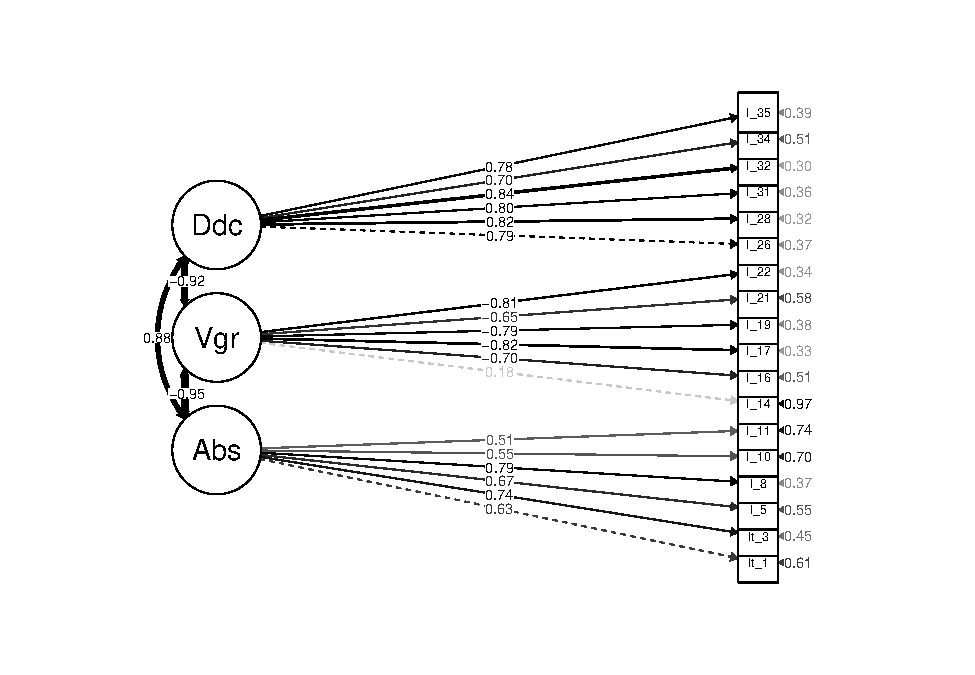
\includegraphics{EngagementPaper2_files/figure-latex/semplotsub-1.pdf}
\caption{\label{fig:semplotsub}Omnibus Confirmatory Factor Analysis substantive structure.}
\end{figure}

\begin{figure}
\centering
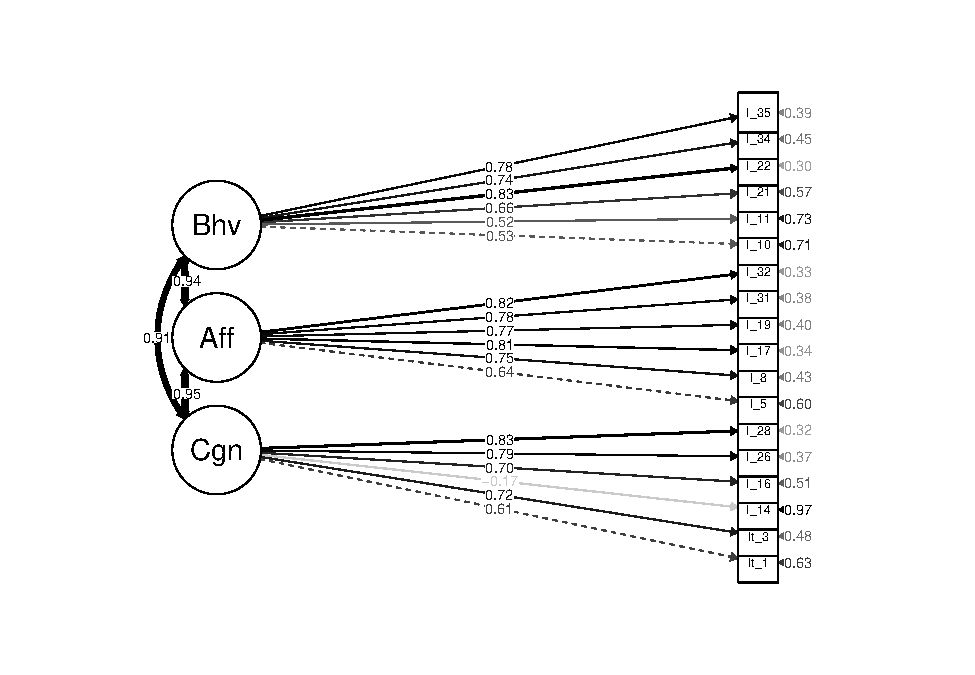
\includegraphics{EngagementPaper2_files/figure-latex/semplotatt-1.pdf}
\caption{\label{fig:semplotatt}Omnibus Confirmatory Factor Analysis attitudinal structure.}
\end{figure}

\begin{longtable}[]{@{}
  >{\raggedright\arraybackslash}p{(\columnwidth - 16\tabcolsep) * \real{0.0670}}
  >{\raggedright\arraybackslash}p{(\columnwidth - 16\tabcolsep) * \real{0.1453}}
  >{\raggedright\arraybackslash}p{(\columnwidth - 16\tabcolsep) * \real{0.1117}}
  >{\raggedright\arraybackslash}p{(\columnwidth - 16\tabcolsep) * \real{0.1229}}
  >{\raggedright\arraybackslash}p{(\columnwidth - 16\tabcolsep) * \real{0.1117}}
  >{\raggedright\arraybackslash}p{(\columnwidth - 16\tabcolsep) * \real{0.1117}}
  >{\raggedright\arraybackslash}p{(\columnwidth - 16\tabcolsep) * \real{0.1061}}
  >{\raggedright\arraybackslash}p{(\columnwidth - 16\tabcolsep) * \real{0.1117}}
  >{\raggedright\arraybackslash}p{(\columnwidth - 16\tabcolsep) * \real{0.1117}}@{}}
\toprule\noalign{}
\begin{minipage}[b]{\linewidth}\raggedright
Condition
\end{minipage} & \begin{minipage}[b]{\linewidth}\raggedright
Model
\end{minipage} & \begin{minipage}[b]{\linewidth}\raggedright
\(\chi^2\)
\end{minipage} & \begin{minipage}[b]{\linewidth}\raggedright
\emph{df}
\end{minipage} & \begin{minipage}[b]{\linewidth}\raggedright
RMSEA
\end{minipage} & \begin{minipage}[b]{\linewidth}\raggedright
SRMR
\end{minipage} & \begin{minipage}[b]{\linewidth}\raggedright
CFI
\end{minipage} & \begin{minipage}[b]{\linewidth}\raggedright
TLI
\end{minipage} & \begin{minipage}[b]{\linewidth}\raggedright
AIC
\end{minipage} \\
\midrule\noalign{}
\endhead
\bottomrule\noalign{}
\endlastfoot
Condition 1 & 3-factor substantive & 300.86 & 132 & 0.14 & 1 & 0.68 & 0.63 & 3,282.88 \\
& 3-factor attitudinal & 290.33 & 132 & 0.14 & 1 & 0.70 & 0.65 & 3,272.35 \\
Condition 2 & 3-factor substantive & 310.01 & 132 & 0.15 & 1 & 0.71 & 0.66 & 3,257.45 \\
& 3-factor attitudinal & 322.52 & 132 & 0.15 & 1 & 0.69 & 0.64 & 3,269.96 \\
Condition 3 & 3-factor substantive & 252.07 & 132 & 0.12 & 1 & 0.78 & 0.74 & 3,510.32 \\
& 3-factor attitudinal & 275.74 & 132 & 0.13 & 1 & 0.73 & 0.69 & 3534 \\
Condition 4 & 3-factor substantive & 224.96 & 132 & 0.10 & 0.94 & 0.82 & 0.79 & 3,421.64 \\
& 3-factor attitudinal & 228.99 & 132 & 0.10 & 0.96 & 0.81 & 0.78 & 3,425.66 \\
Condition 5 & 3-factor substantive & 549.80 & 132 & 0.10 & 1 & 0.90 & 0.89 & 14,932.57 \\
& 3-factor attitudinal & 497.90 & 132 & 0.10 & 1 & 0.92 & 0.90 & 14,880.67 \\
Condition 6 & 3-factor substantive & 468.02 & 132 & 0.09 & 0.87 & 0.91 & 0.90 & 17,953.02 \\
& 3-factor attitudinal & 610.60 & 132 & 0.10 & 1 & 0.88 & 0.86 & 18,095.61 \\
Overall & 3-factor substantive & 930.38 & 132 & 0.08 & 0.76 & 0.92 & 0.90 & 46,884.02 \\
& 3-factor attitudinal & 1,042.75 & 132 & 0.09 & 0.99 & 0.91 & 0.89 & 46,996.40 \\
\end{longtable}

\begin{lltable}

\begin{TableNotes}[para]
\normalsize{\textit{Note.} * p < 0.05; ** p < 0.01; *** p < 0.001}
\end{TableNotes}

\begin{longtable}{llllllll}\noalign{\getlongtablewidth\global\LTcapwidth=\longtablewidth}
\caption{\label{tab:unnamed-chunk-1}Unit-weighted scale intercorrelations (all conditions).}\\
\toprule
 & \multicolumn{1}{c}{1} & \multicolumn{1}{c}{2} & \multicolumn{1}{c}{3} & \multicolumn{1}{c}{4} & \multicolumn{1}{c}{5} & \multicolumn{1}{c}{$M$} & \multicolumn{1}{c}{$SD$}\\
\midrule
\endfirsthead
\caption*{\normalfont{Table \ref{tab:unnamed-chunk-1} continued}}\\
\toprule
 & \multicolumn{1}{c}{1} & \multicolumn{1}{c}{2} & \multicolumn{1}{c}{3} & \multicolumn{1}{c}{4} & \multicolumn{1}{c}{5} & \multicolumn{1}{c}{$M$} & \multicolumn{1}{c}{$SD$}\\
\midrule
\endhead
1. Absorption & - &  &  &  &  & 4.00 & 1.02\\
2. Vigor & .76*** & - &  &  &  & 4.22 & 0.85\\
3. Dedication & .76*** & .79*** & - &  &  & 4.41 & 1.12\\
4. Affect & .81*** & .83*** & .85*** & - &  & 4.08 & 0.90\\
5. Cognition & .87*** & .85*** & .89*** & .79*** & - & 4.16 & 1.12\\
6. Behavior & .84*** & .85*** & .84*** & .73*** & .81*** & 4.39 & 0.96\\
\bottomrule
\addlinespace
\insertTableNotes
\end{longtable}

\end{lltable}

\begin{quote}
Note. Also look at scale intercorrelations when the shared items have been removed (for example, items that define both dedication and cognition when looking at the correlation between dedication and cognition) - 12/2/21
\end{quote}

\hypertarget{condition-effects}{%
\subsubsection{Condition effects}\label{condition-effects}}

The order of item presentation was: 1) random within substantive dimension, 2) random within attitudinal dimension, 3) parcels of substantive within attitudinal (36-item attitudinal context), 4) parcels of attitudinal within substantive (36-item substantive context), 5) parcels of substantive within attitudinal (20-item attitudinal context), and 6) parcels of attitudinal within substantive (20-item substantive context). For example, in condition 1, the first items presented were all associated with one attitudinal dimension (for example, ``Affect''). Once the Affect item list was fully exhausted, the respondent was then administered the full set of Behavioral items, and once these were completed the respondent was then administered the Cognitive item set\footnote{Across conditions, the order of presentation of item ``blocks'' was also randomized. For example, not all respondents in Condition 1 was administered the Affect item block first - roughly 1/3 was presented the Behavioral block first and roughly 1/3 was presented the Cognitive block first.}. We view these orderings as cues regarding factor structure, and anticipated empirical factor structures to reflect these cues. The effects did emerge, but were quite moderate (for example, \(\Delta{\chi^2_{Cond1}}\) = 9.55, \(\Delta{AIC_{Cond1}}\) = 10.53). Given the variety of item orderings administered, this should be considered somewhat comforting regarding the effect of contextual embeddedness within multidimensional inventories. To further explore degree of similarity, we applied explicit tests of measurement invariance.

\hypertarget{measurement-invariance}{%
\paragraph{Measurement invariance}\label{measurement-invariance}}

Because our six conditions were obtained across two different sampling procedures, we apply our analyses of measurement invariance twice - first investigating the four conditions administered within our initial snowball sampling and then secondly also extending to the follow-up Qualtrics panel respondents.

We looked at structural invariance as well as latent means (Meredith, 1993; Steinmetz, Schmidt, Tina-Booh, Wieczorek, \& Schwartz, 2009).

\begin{verbatim}
## Warning in lav_object_post_check(object): lavaan WARNING: covariance matrix of latent variables
##                 is not positive definite in group 2;
##                 use lavInspect(fit, "cov.lv") to investigate.
\end{verbatim}

\begin{verbatim}
## Warning in lav_object_post_check(object): lavaan WARNING: covariance matrix of latent variables
##                 is not positive definite in group 3;
##                 use lavInspect(fit, "cov.lv") to investigate.
\end{verbatim}

\begin{verbatim}
## Warning in lav_object_post_check(object): lavaan WARNING: covariance matrix of latent variables
##                 is not positive definite in group 2;
##                 use lavInspect(fit, "cov.lv") to investigate.
\end{verbatim}

\begin{verbatim}
## Warning in lav_object_post_check(object): lavaan WARNING: covariance matrix of latent variables
##                 is not positive definite in group 3;
##                 use lavInspect(fit, "cov.lv") to investigate.
\end{verbatim}

\begin{verbatim}
## Warning in lav_object_post_check(object): lavaan WARNING: covariance matrix of latent variables
##                 is not positive definite in group 2;
##                 use lavInspect(fit, "cov.lv") to investigate.
\end{verbatim}

\begin{verbatim}
## Warning in lav_object_post_check(object): lavaan WARNING: covariance matrix of latent variables
##                 is not positive definite in group 3;
##                 use lavInspect(fit, "cov.lv") to investigate.
\end{verbatim}

\begin{table}[tbp]

\begin{center}
\begin{threeparttable}

\caption{\label{tab:measinv.pilot.att}Measurement invariance summary statistics (attitudinal structure).}

\begin{tabular}{lllllllll}
\toprule
 & \multicolumn{1}{c}{Df} & \multicolumn{1}{c}{AIC} & \multicolumn{1}{c}{BIC} & \multicolumn{1}{c}{Chisq} & \multicolumn{1}{c}{Chisq diff} & \multicolumn{1}{c}{RMSEA} & \multicolumn{1}{c}{Df diff} & \multicolumn{1}{c}{Pr(>Chisq)}\\
\midrule
configural.a & 528 & 13,645.98 & 14,453.38 & 1,117.59 & NA & NA & NA & NA\\
weak.a & 573 & 13,614.45 & 14,262.50 & 1,176.06 & 58.48 & 0.07 & 45 & 0.09\\
strong.a & 618 & 13,569.48 & 14,058.18 & 1,221.09 & 45.03 & 0.00 & 45 & 0.47\\
strict.a & 672 & 13,538.35 & 13,835.82 & 1,297.96 & 76.87 & 0.08 & 54 & 0.02\\
\bottomrule
\addlinespace
\end{tabular}

\begin{tablenotes}[para]
\normalsize{\textit{Note.} * p < 0.05; ** p < 0.01; *** p < 0.001}
\end{tablenotes}

\end{threeparttable}
\end{center}

\end{table}

\begin{verbatim}
## Warning in lav_object_post_check(object): lavaan WARNING: covariance matrix of latent variables
##                 is not positive definite in group 1;
##                 use lavInspect(fit, "cov.lv") to investigate.
\end{verbatim}

\begin{verbatim}
## Warning in lav_object_post_check(object): lavaan WARNING: covariance matrix of latent variables
##                 is not positive definite in group 3;
##                 use lavInspect(fit, "cov.lv") to investigate.
\end{verbatim}

\begin{verbatim}
## Warning in lav_object_post_check(object): lavaan WARNING: covariance matrix of latent variables
##                 is not positive definite in group 1;
##                 use lavInspect(fit, "cov.lv") to investigate.
\end{verbatim}

\begin{verbatim}
## Warning in lav_object_post_check(object): lavaan WARNING: covariance matrix of latent variables
##                 is not positive definite in group 3;
##                 use lavInspect(fit, "cov.lv") to investigate.
\end{verbatim}

\begin{verbatim}
## Warning in lav_object_post_check(object): lavaan WARNING: covariance matrix of latent variables
##                 is not positive definite in group 1;
##                 use lavInspect(fit, "cov.lv") to investigate.
\end{verbatim}

\begin{verbatim}
## Warning in lav_object_post_check(object): lavaan WARNING: covariance matrix of latent variables
##                 is not positive definite in group 3;
##                 use lavInspect(fit, "cov.lv") to investigate.
\end{verbatim}

\begin{verbatim}
## Warning in lav_object_post_check(object): lavaan WARNING: covariance matrix of latent variables
##                 is not positive definite in group 1;
##                 use lavInspect(fit, "cov.lv") to investigate.
\end{verbatim}

\begin{verbatim}
## Warning in lav_object_post_check(object): lavaan WARNING: covariance matrix of latent variables
##                 is not positive definite in group 4;
##                 use lavInspect(fit, "cov.lv") to investigate.
\end{verbatim}

\begin{table}[tbp]

\begin{center}
\begin{threeparttable}

\caption{\label{tab:measinv.pilot.sub}Measurement invariance summary statistics (substantive structure).}

\begin{tabular}{lllllllll}
\toprule
 & \multicolumn{1}{c}{Df} & \multicolumn{1}{c}{AIC} & \multicolumn{1}{c}{BIC} & \multicolumn{1}{c}{Chisq} & \multicolumn{1}{c}{Chisq diff} & \multicolumn{1}{c}{RMSEA} & \multicolumn{1}{c}{Df diff} & \multicolumn{1}{c}{Pr(>Chisq)}\\
\midrule
configural.s & 528 & 13,616.29 & 14,423.69 & 1,087.90 & NA & NA & NA & NA\\
weak.s & 573 & 13,588.39 & 14,236.44 & 1,150.00 & 62.10 & 0.08 & 45 & 0.05\\
strong.s & 618 & 13,546.51 & 14,035.20 & 1,198.12 & 48.12 & 0.03 & 45 & 0.35\\
strict.s & 672 & 13,521.28 & 13,818.74 & 1,280.89 & 82.77 & 0.09 & 54 & 0.01\\
\bottomrule
\addlinespace
\end{tabular}

\begin{tablenotes}[para]
\normalsize{\textit{Note.} * p < 0.05; ** p < 0.01; *** p < 0.001}
\end{tablenotes}

\end{threeparttable}
\end{center}

\end{table}

\begin{verbatim}
## Warning in lav_object_post_check(object): lavaan WARNING: covariance matrix of latent variables
##                 is not positive definite in group 2;
##                 use lavInspect(fit, "cov.lv") to investigate.
\end{verbatim}

\begin{verbatim}
## Warning in lav_object_post_check(object): lavaan WARNING: covariance matrix of latent variables
##                 is not positive definite in group 3;
##                 use lavInspect(fit, "cov.lv") to investigate.
\end{verbatim}

\begin{verbatim}
## Warning in lav_object_post_check(object): lavaan WARNING: covariance matrix of latent variables
##                 is not positive definite in group 2;
##                 use lavInspect(fit, "cov.lv") to investigate.
\end{verbatim}

\begin{verbatim}
## Warning in lav_object_post_check(object): lavaan WARNING: covariance matrix of latent variables
##                 is not positive definite in group 3;
##                 use lavInspect(fit, "cov.lv") to investigate.
\end{verbatim}

\begin{verbatim}
## Warning in lav_object_post_check(object): lavaan WARNING: covariance matrix of latent variables
##                 is not positive definite in group 2;
##                 use lavInspect(fit, "cov.lv") to investigate.
\end{verbatim}

\begin{verbatim}
## Warning in lav_object_post_check(object): lavaan WARNING: covariance matrix of latent variables
##                 is not positive definite in group 3;
##                 use lavInspect(fit, "cov.lv") to investigate.
\end{verbatim}

\begin{table}[tbp]

\begin{center}
\begin{threeparttable}

\caption{\label{tab:measinv.siop2.att}Measurement invariance summary statistics (attitudinal structure [6 conditions]).}

\begin{tabular}{lllllllll}
\toprule
 & \multicolumn{1}{c}{Df} & \multicolumn{1}{c}{AIC} & \multicolumn{1}{c}{BIC} & \multicolumn{1}{c}{Chisq} & \multicolumn{1}{c}{Chisq diff} & \multicolumn{1}{c}{RMSEA} & \multicolumn{1}{c}{Df diff} & \multicolumn{1}{c}{Pr(>Chisq)}\\
\midrule
configural.a2 & 792 & 46,694.26 & 48,335.92 & 2,226.09 & NA & NA & NA & NA\\
weak.a2 & 867 & 46,713.85 & 47,995.49 & 2,395.68 & 169.59 & 0.09 & 75 & 0.00\\
strong.a2 & 942 & 46,905.27 & 47,826.90 & 2,737.10 & 341.42 & 0.15 & 75 & 0.00\\
strict.a2 & 1032 & 46,946.38 & 47,436.00 & 2,958.21 & 221.11 & 0.10 & 90 & 0.00\\
\bottomrule
\addlinespace
\end{tabular}

\begin{tablenotes}[para]
\normalsize{\textit{Note.} * p < 0.05; ** p < 0.01; *** p < 0.001}
\end{tablenotes}

\end{threeparttable}
\end{center}

\end{table}

\hypertarget{discussion}{%
\section{Discussion}\label{discussion}}

The item cues did provide slight response cues (attending to individual model fit indices), however, the effect was quite small. Measurement invariance is plausible within our initial four administration conditions, although it is not attained across all six conditions. This is possibly attributable to differences in sampled population (in addition to the possibility that this difference is attributable to item orderings).

\newpage

\hypertarget{references}{%
\section{References}\label{references}}

\begingroup
\setlength{\parindent}{-0.5in}
\setlength{\leftskip}{0.5in}

\hypertarget{refs}{}
\begin{CSLReferences}{1}{0}
\leavevmode\vadjust pre{\hypertarget{ref-ackerman1989comparison}{}}%
Ackerman, T. A., Spray, J. A., Reckase, M. D., \& Carlson, J. E. (1989). \emph{A comparison of the effects of random versus fixed order of item presentation via the computer}. AMERICAN COLL TESTING PROGRAM IOWA CITY IA.

\leavevmode\vadjust pre{\hypertarget{ref-baumruk2004missing}{}}%
Baumruk, R. (2004). \emph{The missing link: The role of employee engagement in business success}. \emph{47}, 48--52.

\leavevmode\vadjust pre{\hypertarget{ref-coffman_hard_1999}{}}%
Coffman, C., \& Harter, J. (1999). A hard look at soft numbers. \emph{Position Paper, Gallup Organization}.

\leavevmode\vadjust pre{\hypertarget{ref-cole2012job}{}}%
Cole, M. S., Walter, F., Bedeian, A. G., \& O'Boyle, E. H. (2012). Job burnout and employee engagement: A meta-analytic examination of construct proliferation. \emph{Journal of Management}, \emph{38}(5), 1550--1581.

\leavevmode\vadjust pre{\hypertarget{ref-csikszentmihalyi1990flow}{}}%
Csikszentmihalyi, M. (1990). \emph{Flow: The psychology of optimal experience} (Vol. 1990). Harper \& Row New York.

\leavevmode\vadjust pre{\hypertarget{ref-dean1980presentation}{}}%
Dean, M. L. (1980). Presentation order effects in product taste tests. \emph{The Journal of Psychology}, \emph{105}(1), 107--110.

\leavevmode\vadjust pre{\hypertarget{ref-elloy_examination_1991}{}}%
Elloy, D. F., Everett, J. E., \& Flynn, W. R. (1991). An examination of the correlates of job involvement. \emph{Group \& Organization Studies}, \emph{16}(2), 160--177. \url{https://doi.org/10.1177/105960119101600204}

\leavevmode\vadjust pre{\hypertarget{ref-ferris_added_1984}{}}%
Ferris, R., \& Hellier, P. (1984). Added value productivity schemes and employee participation. \emph{Asia Pacific Journal of Human Resources}, \emph{22}(4), 35--44. \url{https://doi.org/10.1177/103841118402200406}

\leavevmode\vadjust pre{\hypertarget{ref-goering2017not}{}}%
Goering, D. D., Shimazu, A., Zhou, F., Wada, T., \& Sakai, R. (2017). Not if, but how they differ: A meta-analytic test of the nomological networks of burnout and engagement. \emph{Burnout Research}, \emph{5}, 21--34.

\leavevmode\vadjust pre{\hypertarget{ref-hamilton1990self}{}}%
Hamilton, J. C., \& Shuminsky, T. R. (1990). Self-awareness mediates the relationship between serial position and item reliability. \emph{Journal of Personality and Social Psychology}, \emph{59}(6), 1301.

\leavevmode\vadjust pre{\hypertarget{ref-harter_business-unit-level_2002}{}}%
Harter, J. K., Schmidt, F. L., \& Hayes, T. L. (2002). Business-unit-level relationship between employee satisfaction, employee engagement, and business outcomes: A meta-analysis. \emph{Journal of Applied Psychology}, \emph{87}(2), 268.

\leavevmode\vadjust pre{\hypertarget{ref-kahn1990psychological}{}}%
Kahn, William A. (1990b). Psychological conditions of personal engagement and disengagement at work. \emph{Academy of Management Journal}, \emph{33}(4), 692--724.

\leavevmode\vadjust pre{\hypertarget{ref-kahn_psychological_1990}{}}%
Kahn, William A. (1990a). Psychological conditions of personal engagement and disengagement at work. \emph{Academy of Management Journal}, \emph{33}(4), 692--724.

\leavevmode\vadjust pre{\hypertarget{ref-kaiser_campbell_2019}{}}%
Kaiser, F. G., \& Wilson, M. (2019). The {Campbell} {Paradigm} as a {Behavior}-{Predictive} {Reinterpretation} of the {Classical} {Tripartite} {Model} of {Attitudes}. \emph{European Psychologist}, \emph{24}(4), 359--374. \url{https://doi.org/10.1027/1016-9040/a000364}

\leavevmode\vadjust pre{\hypertarget{ref-kim_burnout_2009}{}}%
Kim, H. J., Shin, K. H., \& Swanger, N. (2009). Burnout and engagement: {A} comparative analysis using the {Big} {Five} personality dimensions. \emph{International Journal of Hospitality Management}, \emph{28}(1), 96--104. \url{https://doi.org/10.1016/j.ijhm.2008.06.001}

\leavevmode\vadjust pre{\hypertarget{ref-knowles1988item}{}}%
Knowles, E. S. (1988). Item context effects on personality scales: Measuring changes the measure. \emph{Journal of Personality and Social Psychology}, \emph{55}(2), 312.

\leavevmode\vadjust pre{\hypertarget{ref-krosnick1987evaluation}{}}%
Krosnick, J. A., \& Alwin, D. F. (1987). An evaluation of a cognitive theory of response-order effects in survey measurement. \emph{Public Opinion Quarterly}, \emph{51}(2), 201--219.

\leavevmode\vadjust pre{\hypertarget{ref-kulikowski2017we}{}}%
Kulikowski, K. (2017). Do we all agree on how to measure work engagement? Factorial validity of utrecht work engagement scale as a standard measurement tool--a literature review. \emph{International Journal of Occupational Medicine and Environmental Health}, \emph{30}(2), 161--175.

\leavevmode\vadjust pre{\hypertarget{ref-leiter_areas_2004}{}}%
Leiter, M., \& Maslach, C. (2004). Areas of worklife: A structured approach to organizational predictors of job burnout. In \emph{Research in occupational stress and well-being} (Vol. 3, pp. 91--134). \url{https://doi.org/10.1016/S1479-3555(03)03003-8}

\leavevmode\vadjust pre{\hypertarget{ref-leone_relation_1995}{}}%
Leone, D. R. (1995). \emph{The relation of work climate, higher order need satisfaction, need salience, and causality orientations to work engagement, psychological adjustment, and job satisfaction} (PhD thesis). ProQuest Information \& Learning.

\leavevmode\vadjust pre{\hypertarget{ref-mashburn2014effect}{}}%
Mashburn, A. J., Meyer, J. P., Allen, J. P., \& Pianta, R. C. (2014). The effect of observation length and presentation order on the reliability and validity of an observational measure of teaching quality. \emph{Educational and Psychological Measurement}, \emph{74}(3), 400--422.

\leavevmode\vadjust pre{\hypertarget{ref-maslach1997causes}{}}%
Maslach, C., \& Leiter, M. (1997). What causes burnout. \emph{Maslach C, Leiter MP. The Truth About Burnout: How Organizations Cause Personal Stress and What to Do about It. San Francisco, CA: Josey-Bass Publishers}, 38--60.

\leavevmode\vadjust pre{\hypertarget{ref-maslach_early_2008}{}}%
Maslach, Christina, \& Leiter, M. P. (2008). Early predictors of job burnout and engagement. \emph{Journal of Applied Psychology}, \emph{93}(3), 498--512.

\leavevmode\vadjust pre{\hypertarget{ref-meredith1993measurement}{}}%
Meredith, W. (1993). Measurement invariance, factor analysis and factorial invariance. \emph{Psychometrika}, \emph{58}(4), 525--543.

\leavevmode\vadjust pre{\hypertarget{ref-meyer_three-component_1991}{}}%
Meyer, J. P., \& Allen, N. J. (1991). A three-component conceptualization of organizational commitment. \emph{Human Resource Management Review}, \emph{1}(1), 61--89.

\leavevmode\vadjust pre{\hypertarget{ref-R-base}{}}%
R Core Team. (2021). \emph{R: A language and environment for statistical computing}. Vienna, Austria: R Foundation for Statistical Computing. Retrieved from \url{https://www.R-project.org/}

\leavevmode\vadjust pre{\hypertarget{ref-rosenberg_cognitive_1960}{}}%
Rosenberg, M. J. (1960). Cognitive, affective, and behavioral components of attitudes. In \emph{Attitude organization and change}.

\leavevmode\vadjust pre{\hypertarget{ref-engage_2022}{}}%
Russell, M., Ossorio Duffoo, C., Garcia Prieto Palacios Roji, R., \& Kulas, J. (2022). Development of an intentional bifactor measure of engagement. \emph{The Seattle Edition of SIOP}, 1--14. SIOP.

\leavevmode\vadjust pre{\hypertarget{ref-schaufeli_uwesutrecht_2003}{}}%
Schaufeli, W. B., \& Bakker, A. B. (2003). {UWES}--utrecht work engagement scale: Test manual. \emph{Unpublished Manuscript: Department of Psychology, Utrecht University}, \emph{8}.

\leavevmode\vadjust pre{\hypertarget{ref-schaufeli_measurement_2002}{}}%
Schaufeli, Wilmar B., Salanova, M., González-Romá, V., \& Bakker, A. B. (2002). The measurement of engagement and burnout: A two sample confirmatory factor analytic approach. \emph{Journal of Happiness Studies}, \emph{3}(1), 71--92.

\leavevmode\vadjust pre{\hypertarget{ref-schaufeli2008workaholism}{}}%
Schaufeli, Wilmar B., Taris, T. W., \& Van Rhenen, W. (2008). Workaholism, burnout, and work engagement: Three of a kind or three different kinds of employee well-being? \emph{Applied Psychology}, \emph{57}(2), 173--203.

\leavevmode\vadjust pre{\hypertarget{ref-schaufeli_conceptualization_2010}{}}%
Schaufeli, W., \& Bakker, A. (2010). The conceptualization and measurement of work engagement. In W. Schaufeli, A. Bakker, \& M. Leiter (Eds.), \emph{Work engagement: A handbook of essential theory and research} (pp. 10--24). New York: Psychology Press.

\leavevmode\vadjust pre{\hypertarget{ref-serico2021methodological}{}}%
Serico, J. M., NeMoyer, A., Goldstein, N. E., Houck, M., \& Leff, S. S. (2021). A methodological study of order effects in reporting relational aggression experiences. \emph{Journal of Interpersonal Violence}, \emph{36}(5-6), 2478--2497.

\leavevmode\vadjust pre{\hypertarget{ref-shaw2005engagement}{}}%
Shaw, K. (2005). An engagement strategy process for communicators. \emph{Strategic Communication Management}, \emph{9}(3), 26.

\leavevmode\vadjust pre{\hypertarget{ref-soane2012development}{}}%
Soane, E., Truss, C., Alfes, K., Shantz, A., Rees, C., \& Gatenby, M. (2012). Development and application of a new measure of employee engagement: The ISA engagement scale. \emph{Human Resource Development International}, \emph{15}(5), 529--547.

\leavevmode\vadjust pre{\hypertarget{ref-staw_employee_1994}{}}%
Staw, B. M., Sutton, R. I., \& Pelled, L. H. (1994). Employee positive emotion and favorable outcomes at the workplace. \emph{Organization Science}, \emph{5}(1), 51--71.

\leavevmode\vadjust pre{\hypertarget{ref-steinberg1994context}{}}%
Steinberg, L. (1994). Context and serial-order effects in personality measurement: Limits on the generality of measuring changes the measure. \emph{Journal of Personality and Social Psychology}, \emph{66}(2), 341--349.

\leavevmode\vadjust pre{\hypertarget{ref-steinmetz2009testing}{}}%
Steinmetz, H., Schmidt, P., Tina-Booh, A., Wieczorek, S., \& Schwartz, S. H. (2009). Testing measurement invariance using multigroup CFA: Differences between educational groups in human values measurement. \emph{Quality \& Quantity}, \emph{43}(4), 599--616.

\leavevmode\vadjust pre{\hypertarget{ref-taris2017burnout}{}}%
Taris, T. W., Ybema, J. F., \& Beek, I. van. (2017). Burnout and engagement: Identical twins or just close relatives? \emph{Burnout Research}, \emph{5}, 3--11.

\leavevmode\vadjust pre{\hypertarget{ref-timms2012burnt}{}}%
Timms, C., Brough, P., \& Graham, D. (2012). Burnt-out but engaged: The co-existence of psychological burnout and engagement. \emph{Journal of Educational Administration}, \emph{50}(3), 327--345.

\leavevmode\vadjust pre{\hypertarget{ref-weinberg2018measurement}{}}%
Weinberg, M. K., Seton, C., \& Cameron, N. (2018). The measurement of subjective wellbeing: Item-order effects in the personal wellbeing index---adult. \emph{Journal of Happiness Studies}, \emph{19}(1), 315--332.

\end{CSLReferences}

\endgroup


\end{document}
